	\subsection{Taxonomy of virtualization by \textit{Bugnion}}
	
	\begin{figure}[H]
		\centering
		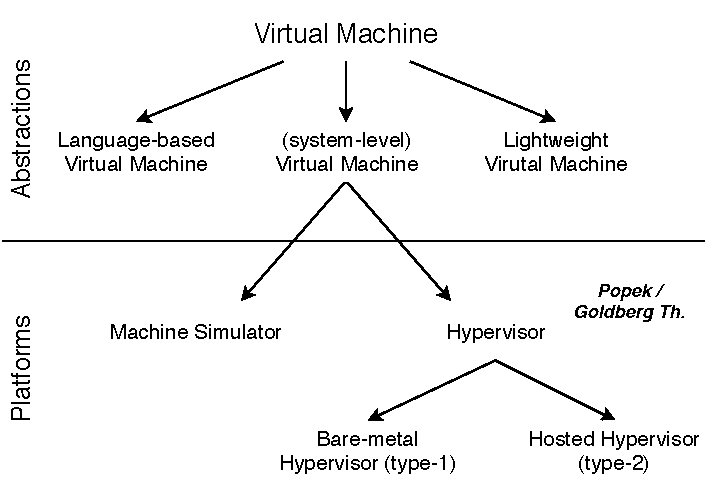
\includegraphics[width=8.5cm]{images/Bugnion2017.pdf}
		\vspace{-0.2cm}
		\caption{Basic classification of virtual machines and the platforms that run them by \textit{Edouard Bugnion, Jason Nieh, Dan Tsafrir and Margaret Martonosi} in 2017 \cite{Bugnion2017}.}
		\label{fig:TaxonomyOfVirtualizationBugnion}
	\end{figure}
	   
    In the \textit{Bugnion et al.}'s study \cite{Bugnion2017}, there is an interesting structure with two level that show the concepts related with the virtual machines. The first level is related with \textit{Abstraction} and its include the categories \textit{Language-base Virtual Machine}, \textit{System-level Virtual Machine}, and \textit{Lightweight Virtual Machine}. The second level is related with \textit{Platform} and its include two categories derivative from \textit{System-level Virtual Machine} called \textit{Machine Simulator}, and \textit{Hypervisor}. The latter, is divided in \textit{Bare-metal Hypervisor} also called \textit{Type-1}, and \textit{Hosted Hypervisor} also called \textit{Type-2}.
    
    
    
    Although,  ...
  
